We based our segmentation approach on DeepLabV3+ using ResNet18 as a backbone and perform the traininig in matlab. 
We combine four existing datasets: hand gesture dataset, hand over face dataset, egohand dataset and GTEA dataset. The resulting dataset was cleaned by removing images containing arm parts and test set images. Our final dataset is composed by 1003 images.
The loss function employed in this project is the dice loss.
\section{Data Augmentation}
We use a data augmentation technique with the aim of increasing the size of the starting dataset and therefore increasing the performance of the classification system. We use both shape-based and color-based transformation and in particular eleven artificial images are created for each image in the dataset. \newline The operations performed are:
\begin{enumerate}
    \item The image is displaced to the right or the left.
    \item The image is displaced up or down.
    \item The image is rotated by an angle randomly selected from the range [0° 180°].
    \item Horizontal or vertical shear by using the function \textit{randomAffine2d}.
    \item Horizontal or vertical flip.
    \item Change in the brightness levels by adding the same value to each RGB channel.
    \item Change in the brightness levels by adding different values to each RGB channel.
    \item Add speckle noise by using the function \textit{imnoise}.
    \item  Convertion of the truecolor image RGB to the grayscale image.
    \item Application of the technique “Contrast and Motion Blur”, described below. 
    \item Application of the technique “Shadows”, described below. 
\end{enumerate}
\subsection{Contrast and Motion Blur}
This transformation is the composition of two alterations: firstly, it is necessary to modify the contrast of the original image, increasing or decreasing it, then a filter that simulates the movement of the camera is applied. Two functions to modify the contrast are implemented, but only one randomly chosen between the two is applied to the image.
The first contrast function is based on the following equation:
\[
	\frac{(x-\frac{1}{2})\sqrt{1-\frac{k}{4}}}{\sqrt{1-k(x-\frac{1}{2}})^2} + 0.5,  k\leq4
	\]
The parameter $k$ controls the contrast, there is an increase in contrast if $k<0$, a decrease in contrast if $0<k\leq4$, the image remains the same when 
$k=0$.
In the code, k is chosen randomly from a specific range, randomly chosen among the following four:
\begin{itemize}
    \item U(2.8, 3.8) $\to$ Hard decrease in contrast.
    \item U(1.5, 2.5) $\to$ Soft decrease in contrast.
    \item U(-2, -1) $\to$ Soft increase in contrast.
    \item U(-5, -3) $\to$ Hard increase in contrast.
\end{itemize}
The second contrast function is based on the following equation:

\[
y =
\left\{
\begin{array}{
  @{}% no padding
  l@{\quad}% some padding
  r@{}% no padding
  >{{}}r@{}% no padding
  >{{}}l@{}% no padding
}
  \frac{1}{2} (\frac{x}{0.5})\alpha,    &   0\leq x <\frac{1}{2}\\
  1 - \frac{1}{2} (\frac{1-x}{0.5})\alpha,    &   \frac{1}{2} \leq x \leq 1\\
\end{array}
\right.
\]
The parameter $\alpha$ controls the contrast, there is an increase in contrast if $\alpha > 1$ , a decrease in contrast if $0 < \alpha < 1$ and the image remains the same when $\alpha = 1$. This parameter is chosen randomly from four possible ranges:
\begin{itemize}
    \item U(0.25, 0.5) $\to$ Hard decrease in contrast.
    \item U(0.6, 0.9) $\to$ Soft decrease in contrast.
    \item U(1.2, 1.7) $\to$ Soft increase in contrast.
    \item U(1.8, 2.3) $\to$ Hard increase in contrast.
\end{itemize}

\subsection{Shadows}
The final image is obtained by applying a shadow  to the left or the right of the original image. In particular, the intensities of the columns are multiplied by the following equation:
\[
y =
\left\{
\begin{array}{
  @{}% no padding
  l@{\quad}% some padding
  r@{}% no padding
  >{{}}r@{}% no padding
  >{{}}l@{}% no padding
}
  \text{min}\left\{0.2 + 0.8 \sqrt{\frac{x}{0.5}}, 1\right\}    &   direction = 1\\
  \text{min}\left\{0.2 + 0.8 \sqrt{\frac{1- x}{0.5}}, 1\right\}    &   direction = 0\\
\end{array}
\right.
\]
\begin{figure}
  \centering
  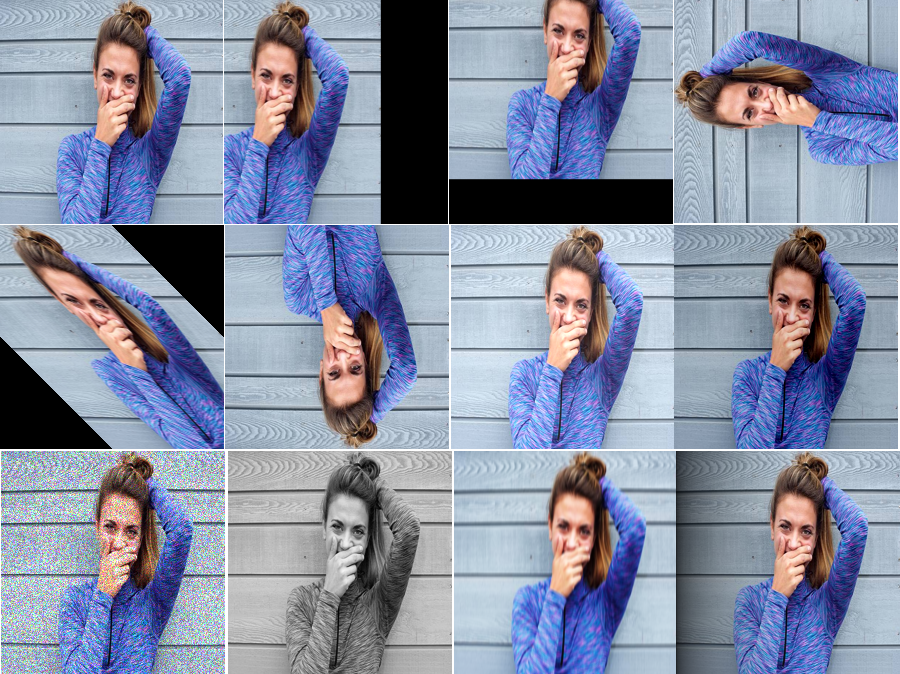
\includegraphics[width=13cm]{images/Immagine.png}
  \caption{The original image (top left) and the artificial images.}
  \label{fig:f01}
\end{figure}
\pagebreak
\section{Unused segmentation}

Before we decide to implement the segmentation using a CNN we try to investigate how to solve the problem using only the OPENCV library method.
We spent a lot of time trying to implement such a solution, so we want to dedicate a little section in our report to details how far we were able to arrive, and the problems that made us change direction.

After many tries we found a solution that basically consist in:
\begin{enumerate}
    \item Application of bilateral filter to the image to smooth the image

    \item Applying a single pixel (threshold) operation to remove pixels that we are sure to not be skin pixels, and color them black. If you are outside this range we discard this pixel and color it black. 
    
    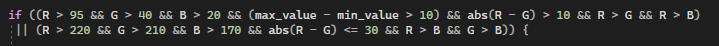
\includegraphics[scale=0.9]{images/unused_seg/code.PNG}
    \newline
    where B is the blue channel, R is the red channel and G is the green channel. max value and min value are respectively the max and min among the R,G,B values.\newline All the details and the motivation behind this choice are explained \href{https://www.researchgate.net/publication/258333832_An_Appropriate_Color_space_to_Improve_Human_Skin_Detection}{here}
    
    \item From the filtered image, we apply a findContours function to find areas (not too big) surrounded by black pixels and discard also the pixel contained in the area.
\end{enumerate}
Since this section wants to give an idea of what we have done, the function that eliminates the background can work on images of arbitrary size, so we may have a more precise result applying the filter on just the portion of image inside the bounding boxes where hands are located, but to understand better the results given by the filter we are just applying it to the whole image.
We now display and comment the results obtained:
First of all, we can say that for an image with a background with color different from skin the filter works well.
\begin{center}
    \begin{figure}[!htb]
        \begin{minipage}{0.5\textwidth}
            \centering
            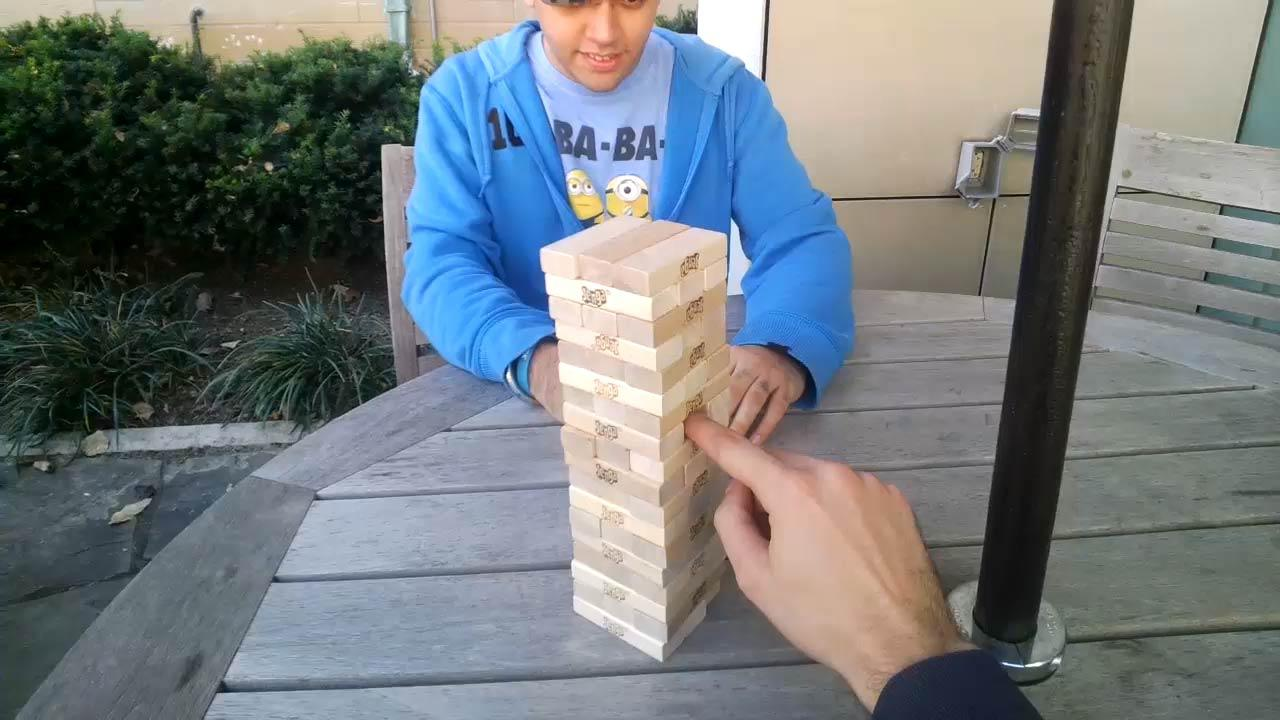
\includegraphics[scale=0.21]{images/unused_seg/20.jpg}
        \end{minipage}
        \begin{minipage}{0.5\textwidth}
            \centering
            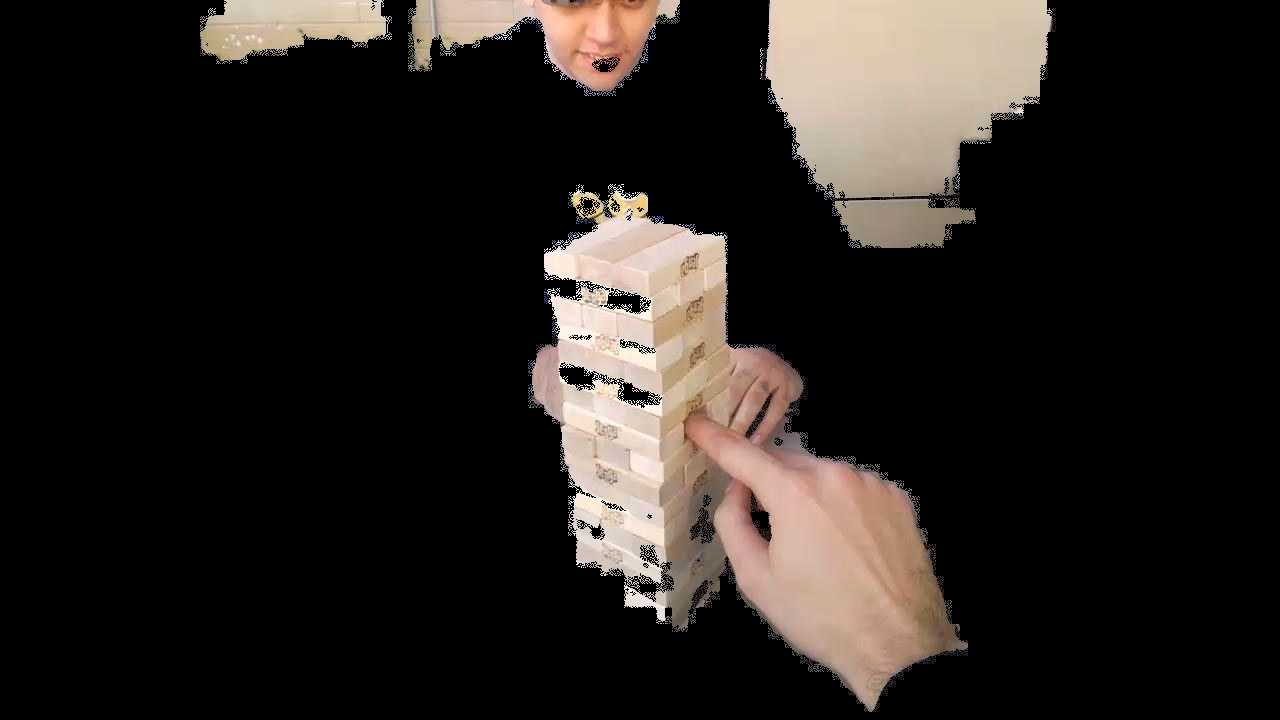
\includegraphics[scale=0.21]{images/unused_seg/20m.jpg} 
        \end{minipage}
    \end{figure}
\end{center}
Applying the filter to this image creates a very good result, applying the image only on bounding box portion would create an almost perfect segmentation of the hand (Based obviously on the accuracy of the bounding box, but we can state that with a good “cut” we can create an image with the full hand colored plus some piece of “Jenga” contained in the , which is perhaps impossible to eliminate since is almost the same color of the hand).
\newline
Another important pros of our filter is that it works well with different skin tone:

\begin{center}
    \begin{figure}[!htb]
        \begin{minipage}{0.5\textwidth}
            \centering
            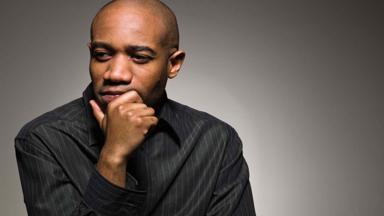
\includegraphics[scale=0.7]{images/unused_seg/30.jpg}
        \end{minipage}
        \begin{minipage}{0.5\textwidth}
            \centering
            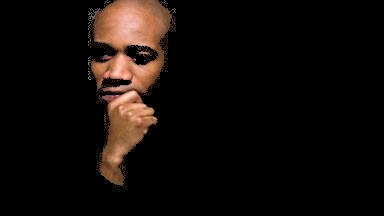
\includegraphics[scale=0.7]{images/unused_seg/30m.jpg} 
        \end{minipage}
    \end{figure}
\end{center}
\pagebreak
Talking about cons of our application we have a strong sensitive to shady portion of hands: 

\begin{center}
    \begin{figure}[!htb]
        \begin{minipage}{0.5\textwidth}
            \centering
            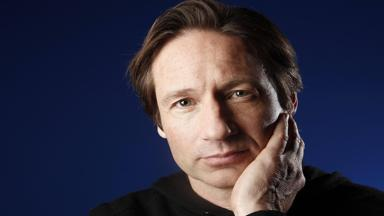
\includegraphics[scale=0.7]{images/unused_seg/21.jpg}
        \end{minipage}
        \begin{minipage}{0.5\textwidth}
            \centering
            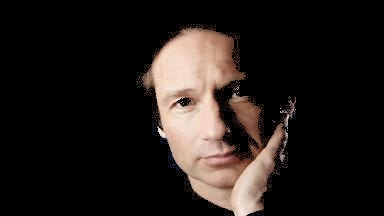
\includegraphics[scale=0.7]{images/unused_seg/21m.jpg} 
        \end{minipage}
    \end{figure}
\end{center}
As you can see clearly from the image above, basically all the parts of the hand that are “in the shade” are eliminated, and unfortunately, using a more permissive threshold would allows shady part of images but also other parts of the background which would be labelled wrongly. The threshold used is one of the best trade-off between false positive and false negative that we were able to find. 
The last but not least big problem that we recognized, and you can also see from the images above is the impossibility to eliminate the other “skin part” of a person, like arms or faces:

\begin{center}
    \begin{figure}[!htb]
        \begin{minipage}{0.5\textwidth}
            \centering
            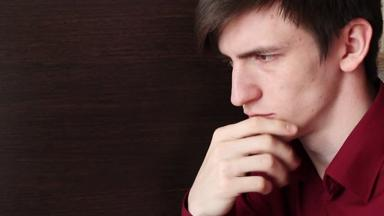
\includegraphics[scale=0.7]{images/unused_seg/28.jpg}
        \end{minipage}
        \begin{minipage}{0.5\textwidth}
            \centering
            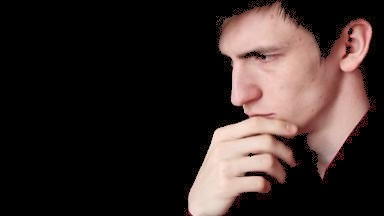
\includegraphics[scale=0.7]{images/unused_seg/28m.jpg} 
        \end{minipage}
    \end{figure}
\end{center}

\begin{center}
    \begin{figure}[!htb]
        \begin{minipage}{0.5\textwidth}
            \centering
            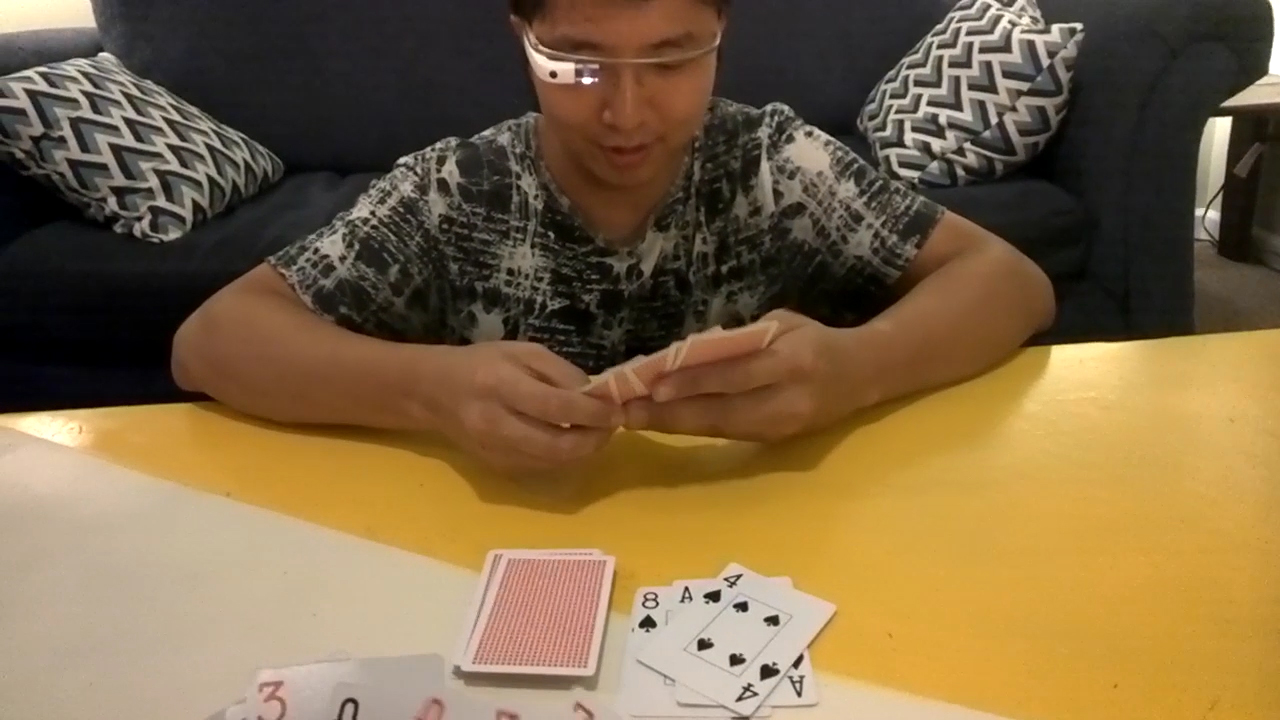
\includegraphics[scale=0.21]{images/unused_seg/8.jpg}
        \end{minipage}
        \begin{minipage}{0.5\textwidth}
            \centering
            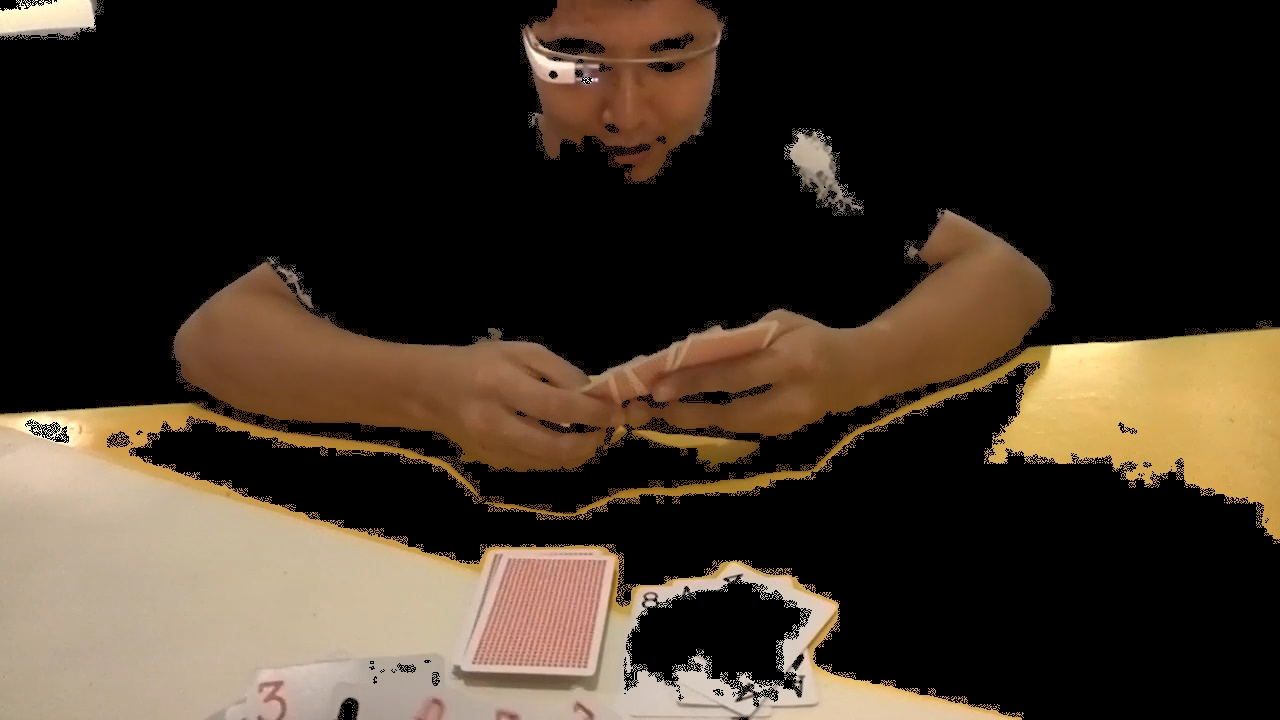
\includegraphics[scale=0.21]{images/unused_seg/8m.jpg} 
        \end{minipage}
    \end{figure}
\end{center}
As you can see here the filter application (even in the portion of bounding box) would color not only the hand but also all the other portion of the skin inside the image, and this lend to a poor result for many of the “Hand over faces” images and for the images where arms is not covered.
\break
\newline
Now to let the reader understand what would be an hypothetical result applying our filter to a bounding box we display a sample using a "perfect" bounding-box from “Hands over face” dataset, and one can note that it doesn’t lead to a good solution. This time, instead of displaying the discarded pixel as black, we will display the image segmented coloring the pixel belonging to the mask (In red)  
\begin{center}
    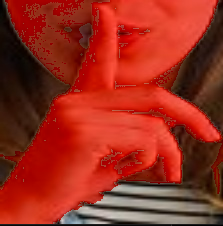
\includegraphics[scale=1.2]{images/unused_seg/output105.PNG}
\end{center}
\noindent
The problems related to shady parts and other skin parts of the image plus the fact that we cannot guarantee that we would apply the segmentation on a good bounding box let this solution being too situational and doesn’t guarantee any “lower bound” of quality for the image segmentation. This forces us to search for a better solution.
